\documentclass{beamer}
\usefonttheme{serif}
\usecolortheme[named=black]{structure}
\setbeamertemplate{footline}[frame number]{}
\setbeamertemplate{navigation symbols}{}

\usepackage[normalem]{ulem} % underlining

% LANGUAGE + FONT
		    
\usepackage[english]{babel}

\usepackage{natbib}
\bibpunct[: ]{[}{]}{;}{a}{}{,}
\bibliographystyle{rusnat}

\usepackage{fontspec}  
\setmainfont{Gentium Plus}


% DRAWING

\usepackage{tikz}
\usepackage{tikz-qtree}
\usetikzlibrary{shapes.geometric}
\usetikzlibrary{trees,arrows}
\usetikzlibrary{positioning}

% LINGUISTICS 

%\usepackage{gb4e}
\usepackage{expex}
\lingset{aboveglftskip=0ex, belowglpreambleskip=0ex, belowexskip=1ex, aboveexskip=1ex, interpartskip=1ex}

\gathertags
\usepackage[glossaries]{leipzig}
\newleipzig{freq}{freq}{Frequentative}
\newleipzig{add}{add}{Additive particle}
\newleipzig{nfin}{nfin}{Non-Finite}
\newleipzig{npst}{npst}{Non-Past}
\newleipzig{int}{int}{Intensifier}
\newleipzig{pssg}{poss.2sg}{Discoursive non-possessive}
% \makeglossaries

\usepackage{stmaryrd}

\usepackage[linguistics]{forest}

% MATH
\usepackage{amssymb}

\title{(Ад)номинальный интенсификатор: случай северного хантыйского}
\author{Аркадий Шалдов \inst{1} \and Алексей Козлов \inst{1, 2}}
\institute{\inst{1} НИУ ВШЭ, \inst{2} ИЯз РАН}
\date{ТМП, Москва, 11.10.23}

\begin{document}

\newcommand{\colone}[1]{\textcolor{red}{#1}}
\newcommand{\coltwo}[1]{\textcolor{blue}{#1}}

\AtBeginSubsection[]
{
    \begin{frame}
        \frametitle{Table of Contents}
        \tableofcontents[currentsection,currentsubsection]
    \end{frame}
}

% -------------------------- текстиктекстиктекстик -----------------------------

\begin{frame}
    \titlepage
\end{frame}

\begin{frame}
    \frametitle{TOC}
    
    \tableofcontents
    
\end{frame}

\section{О чем это мы}

\begin{frame}
    \frametitle{О данных}
    
    Казымский < северный хантыйский < обско-угорские < уральские\\~\\
    
    Данные собраны с помощью элицитации в 2019—2023 во время экспедиций в сёла Казым, Помут и Нумто (Белоярский район, ХМАО)
    
\end{frame}

\subsection{О неограниченном прономинале в северном хантыйском}

\begin{frame}
    \frametitle{\textit{λʉw}: первое знакомство}
    
    \begin{columns}
        \begin{column}{0.5\textwidth}
            Местоименная парадигма из
            \begin{itemize}
                \item 3 лиц
                \item 3 чисел
                \item 3 падежей: NOM, ACC, DAT
                \begin{itemize}
                    \item не имеют падежа LOC, маркирующего также инструмент и пассивного агенса
                \end{itemize}
            \end{itemize}
        \end{column}

        \begin{column}{0.5\textwidth}
            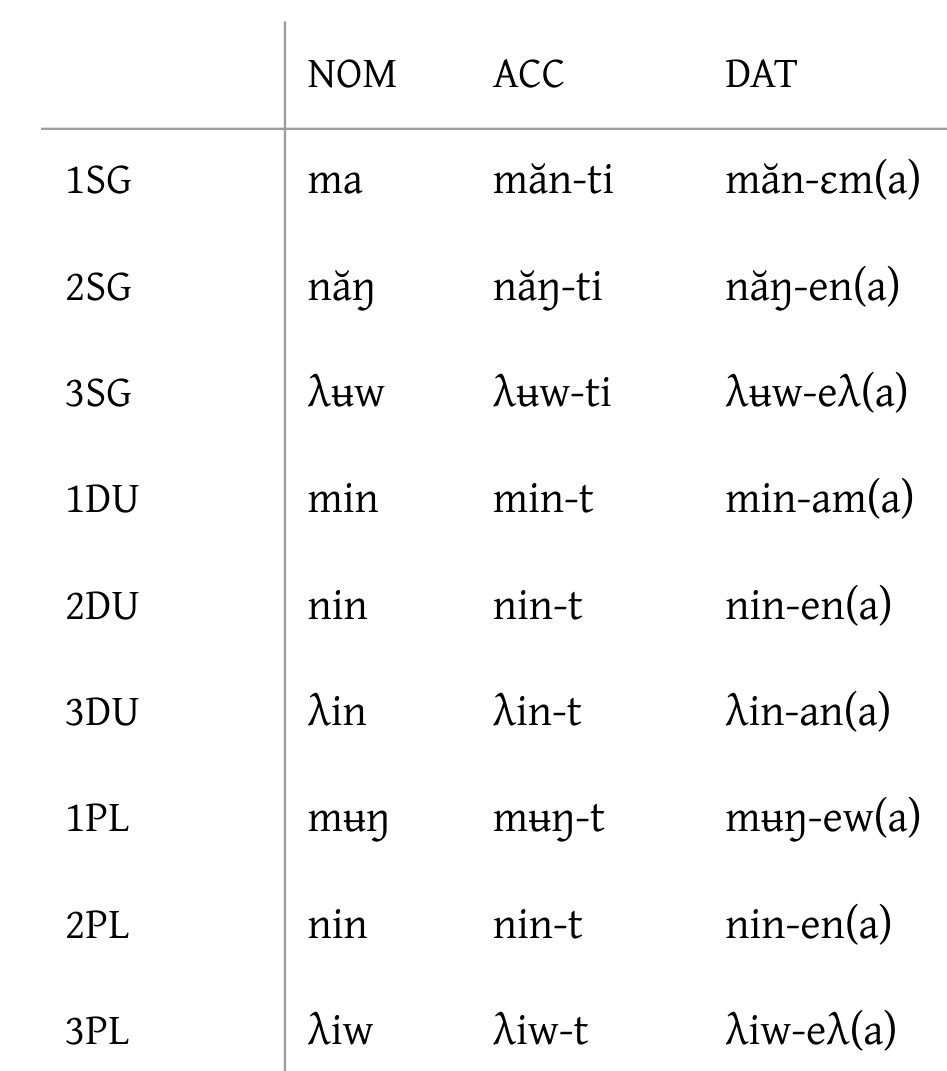
\includegraphics[width = \textwidth]{paradigm.png}
        \end{column}
    \end{columns}
    
\end{frame}

\begin{frame}
    \frametitle{\textit{λʉw}: анафор и рефлексив}
    
    От локального до дейктического контекста 
    
    \ex<refl>
    \begingl
    \gla waśkaj-en$_i$		\textbf{λʉw-ti}$_{i/j}$	išək-s-əλλe//
    \glb В.-\Pssg{} 	\Int-ACC 	хвалить-\Pst{}-\Tsg{}>\Sg{}//
    \glft 1. ‘Вася похвалил  себя’\\
    2. (указ.) ‘Вася похвалил его (не Васю)’//
    \endgl        
    \xe
    
    \ex<ana>
    \begingl
    \glpreamble ‘Там был хороший учитель, Молданов Максим Тимофеевич’//
    \gla i	\textbf{λʉw}		juχt-ijλ-s,				iśi	lupəs				mʉŋ-ewa//
    \glb и 	он(а) 	прийти-FREQ-PST[3SG], 	тоже говорить-PST[3SG] 	мы-DAT//
    \glft ‘Он тоже приходил, тоже с нами разговаривал.’//
    \endgl
    \xe
    
\end{frame}

\begin{frame}
    \frametitle{\textit{λʉw} значит очень много}

    \begin{itemize}
        \item Засвидетельствована ли где-то еще полисемия типа прономинал+рефлексив+интенсификатор? 
        \item На первый взгляд, такое совпадение есть в цахурском (А. Е. Кибрик (ред.) 1999 ) 
        \item Тем не менее, в цахурском это маркированное средство дискурсивной анафоры (ориентированное на фокус эмпатии), а в хантыйском — дефолтное
        \item Эта полифункциональность типологически неожиданна ([Kiparsky 2002]; [Huang 2000]) 
    \end{itemize}

\end{frame}

\subsection{Об интенсификаторах}
        \begin{frame}
            \frametitle{Введение: интенсификаторы}
            
            Фокусные выражения, которые вызывают контраст индивида со связанными с ним каким-нибудь салиентным отношением\\~\\
            
            Адноминальные
            \pex
            \a Васина собака несколько смышленнее \textbf{самого} Васи \textbf{himself}. (Вася vs Васина собака)
            \a Даже \textbf{сама} докладчица не верила в представленную гипотезу. (докладчица vs оппоненты докладчицы)
            \xe
            
            \only<1>{
            Адвербиальные (нас сегодня не интересуют)
            \ex
            Валентина Тимуровна пересекла дорогу \textbf{сама}. (без чьей-либо помощи)
            \xe}
            
            \pause
            
            ~\\~\\Анализ Регины Эккардт [Eckardt 2001]:
            
            \begin{itemize}
                \item интенсификатор --- функция идентичности $\lambda x \in D_e. ID(x)$
                \item всегда в фокусе — в противном случае не привносит значения
                \item фокусные альтернативы [Rooth 1992] — функции отношения (собака-принадлежащая-x, оппоненты-x и пр.)
            \end{itemize}

            
        \end{frame}

        \begin{frame}
    \frametitle{Значения интенсификаторов}
    
    Значения приименных интенсификатор можно поделить так [Lyutikova 2001, Eckardt 2001]:
    
    \begin{itemize}
        \item противительное: \textit{Это сделал не Васин брат, а \textbf{сам} Вася.}
        \item добавочное: \textit{Вася \textbf{сам} был не против жестокого обращения с его данными.}
        \item контрастивно топикальное: \textit{Васина жена ушла, а \textbf{сам} Вася остался.}
        \item скалярное: \textit{Встречу посетил \textbf{сам} проректор.}
    \end{itemize}
    
\end{frame}

\section{\textit{λʉw}}

\subsection{\textit{λʉw} как интенсификатор}

\begin{frame}
    \frametitle{\textit{λʉw}: интенсификатор}

    \textit{λʉw} употребляется как интенсификатор — в противительном и добавочном значениях.
    
    \ex<base1> \begingl
        \glpreamble \{Это Васин брат в снегу лежит?\}//
        \gla ăntɵ śit waśaj-en \textbf{λʉw} u-λ//
        \glb нет это Вася-\Pssg{} \Int{} лежать-\Npst{}//
        \glft 'Нет, это сам Вася лежит.'//
    \endgl    
    \xe
    \ex<base2> \begingl
        \glpreamble \{А правда, Пашина жена не хочет заводить собаку?\}//
        \gla pašaj-en \textbf{λʉw} ănt λăŋχa-λ amp tăj-ti//
        \glb Паша-\Pssg{} \Int{} \Neg{} хотеть-\Npst{} собака заводить-\Nfin.\Npst{}//
        \glft 'Паша и сам не хочет заводить собаку.'//
    \endgl    
    \xe
    
\end{frame}

\begin{frame}
    \frametitle{интенсификатор: сочетаемость}

    Интенсификатор несовместим с прономиналом

    \ex<intpro>
        \begingl
            \gla λʉw		(*λʉw)	at	juχət-λ//
            \glb \Int{}	\Int{}	пусть	прийти-\Npst//
            \glft ожид. ‘Пусть он сам придет.’//
        \endgl
    \xe

    Поэтому с 1 и 2 лицом интенсификатор, как правило, невозможен:

    \ex<intpropro>
        \begingl
            \gla ma	(*ma)		juχət-λ-əm            //
            \glb я	я		прийти-NPST-1SG            //
            \glft             ‘Я сам пришел.’//
        \endgl
    \xe
\end{frame}

\begin{frame}
    \frametitle{Скалярное прочтение}

    При скалярном прочтении интенсификаторов пресуппонируется высокое положение индивида на (достаточно фиксированной) шкале \textbf{ранга}.

    \only<1>{
    \ex<scalru>
        Встречу посетил \textbf{сам} проректор.
    \xe}

    \pause

    ~\\В скалярном прочтении интенсификатор невозможен\\~\\
        
    \ex<foc>\begingl
    \gla\ljudge{*}president \textbf{λʉw} waśaj-en sawot kɵšaj-a oməs-s-əλλe//
    \glb президент \Int{} Вася-\Pssg{} завод глава-\Dat{} ставить-\Pst{}-\Tsg{}>\Sg{}//
    \glft ожид. 'Сам президент назначил Васю главной завода.'//
    \endgl
    \xe

    \pause

    \begin{itemize}
        \item \textbf{Предположение}. В скалярном прочтении интенсифицируемое фокусно. \textit{λʉw} требует топикального интенсифицируемого.
    \end{itemize}
\end{frame}

\subsection{\textit{λʉw} и его сложные отношения с контрастивным топиком}

\begin{frame}
    \frametitle{Контрастивный топик}

    Приименные интенсификаторы обычно могут употребляться не только в позиции фокуса, но и в позиции контрастного топика (для его описания тоже нужны альтернативы [Büring 2014])

    \pex<ctru>
        \a<de>Der König \uppercase{selbst}/ trug ein \uppercase{kro}ne\textbackslash{} [Eckardt 2001: 387]
        \a<en> The king himSELF/ wore a CROwn\textbackslash
        \a<ru> На саМОМ / короле была коРОна \textbackslash
    \xe

    \textit{λʉw} употребляется в позиции КТ ограниченно
    

\end{frame}

\begin{frame}    


    \frametitle{Контрастивный топик}

    Обычно контрастивные топики [Büring 2014] лицензируются в парной структуре:
    \begin{itemize}
        \item \colone{CT1} … \coltwo{F1}
        \item \colone{CT2} … \coltwo{F2}
    \end{itemize}

    \pex
        \a \colone{[Маша]$_{\text{CT1}}$} ест \coltwo{[кашу]$_{\text{F1}}$}, а \colone{[Вася]$_{\text{CT2}}$} ест \coltwo{[суп]$_{\text{F2}}$}
        \a Вася \colone{[сам]$_{\text{CT1}}$} ест \coltwo{[кашу]$_{\text{F1}}$}, а Васины \colone{[приспешники]$_{\text{CT2}}$} едят \coltwo{[суп]$_{\text{F2}}$}
        \a Васины \colone{[приспешники]$_{\text{CT1}}$} едят \coltwo{[кашу]$_{\text{F1}}$}, а \colone{[сам]$_{\text{CT2}}$} Вася ест \coltwo{[суп]$_\text{{F2}}$}
    \xe
    
    \textit{λʉw}-интенсификатор не может быть \coltwo{CT2}

\end{frame}

\begin{frame}
    \frametitle{Контрастивный топик}
    
    \ex<ct2>
    \begingl
        \gla kol’a-jen \textbf{λʉw} sora juχi juχtəs, + kol’a-jen imeλ λońś-a roχanλ-əm-aλ//
        \glb К.-\Pssg{}  \Int{} быстро назад прийти-\Pst, К. жена снег-\Dat{} упасть-\Nfin.\Npst-\Poss{}.\Tsg{} //
        \glft ‘Сам Коля быстро вернулся, а Колина жена провалилась в сугроб’//
    \endgl
    \xe
    
    \pause
    но
    
    \ex<ct>
        \begingl
            \gla kol’a-jen imeλ sora juχi juχtəs, + kol’a-jen (\#\textbf{λʉw}) λońś-a roχanλ-əm-aλ//
            \glb К.-\Pssg{}  жена быстро назад прийти-\Pst, К. \Int{} снег-\Dat{} упасть-\Nfin.\Npst-\Poss{}.\Tsg{} //
            \glft ожид. ‘Колина жена быстро вернулась, а сам Коля провалился в сугроб’//
        \endgl
    \xe


\end{frame}


\begin{frame}
    \frametitle{Контрастивный топик: объяснение}

    \begingl
        \gla \phantom{}[kol’a-jen]$_\text{\textbf{TOP}}$ [\textbf{λʉw}]$_\text{CT}$ [sora juχi juχtəs]$_\text{F}$//
        \glb К.-\Pssg{}  \Int{} быстро назад прийти-\Pst//
        \glft ‘Сам Коля быстро вернулся'//
    \endgl

    ~\\\begin{itemize}
        \item Что за составляющая перед контрастивным топиком?
        \pause
        \item Заякоривающий (anchoring) топик, активирующий полуактивированного участника
        \pause
        \item Rizzi 1997: топиков может быть много
    \end{itemize}

\end{frame}

\begin{frame}
    \frametitle{Контрастивный топик: объяснение}

    \ex<ct>
        \begingl
            \gla kol’a-jen imeλ sora juχi juχtəs, + kol’a-jen (\#\textbf{λʉw}) λońś-a roχanλ-əm-aλ//
            \glb К.-\Pssg{}  жена быстро назад прийти-\Pst, К. \Int{} снег-\Dat{} упасть-\Nfin.\Npst-\Poss{}.\Tsg{} //
            \glft ожид. ‘Колина жена быстро вернулась, а сам Коля провалился в сугроб’//
        \endgl
    \xe

    \begin{itemize}
        \item Во второй клаузе референта ИГ kol’a-jen не нужно активировать: полная ИГ была в первой клаузе
        \item Без полной ИГ во второй клаузе получается нужное прочтение
    \end{itemize}

\end{frame}

\begin{frame}
    \frametitle{Интенсификатор без интенсификатума}

    \ex
    \begingl
        \gla mašaj-en		aŋki	uš-a		wɛr-s-əm,	∅	λʉw-ti		śit	ăntɵ//
        \glb Маша-\Poss.\Ssg{}	мать ус-\Dat{} делать-\Pst-\Fsg{}	pro \Int{}-\Acc{}	\Dem{}	\Neg{}//
        \glft 'Машину мать я узнал, а ее саму нет.'//
    \endgl
    \xe

    ~\\Ср. рус. \textit{\#Машину$_i$ мать я узнал, а её$_i$ – нет}

\end{frame}

\begin{frame}
    \frametitle{Интенсификатор без интенсификатума}

    \ex
    \begingl
        \gla măn-ɛm pewəλ-ti χʉś-s-ən, + λɵmət-suχ-λ-am năŋ λɵmət-s-əλλan //
        \glb я-\Dat{} купаться-\Nfin.\Npst{} манить-\Pst-\Ssg{} одежда-\Pl-\Fsg{} ты одеть-\Pst-\Ssg>\Pl{}        //
        \glft ‘Ты позвала меня купаться, а сама мою одежду одела’\trailingcitation{[Дядюн 2016]}//
    \endgl
    \xe

\end{frame}

\begin{frame}
    \frametitle{Контрастивный топик: объяснение}

    \begin{itemize}
        \item “Дискурсивное” значение (возможность употребляться в контрастивном топике) всё же есть
        \item По независимым причинам при дискурсивном значении невозможно выразить интенсификат
        \item В отсутствие интенсификата неясно, не анафорическое ли это \textit{λʉw}
    \end{itemize}
\end{frame}


\subsection{\textit{λʉw} и его избирательный вкус к синтаксическим позициям}

\begin{frame}
    \frametitle{Казалось бы}

    \textit{λʉw} — \textbf{приименной} интенсификатор\\~\\
    
    Он находится внутри DP, и внешний синтаксис этой DP не должен на него влиять\\~\\
    
    \pause
    
    \onslide{Но это не так}
    
    \begin{itemize}
        \item \textit{λʉw} может ассоциироваться только субъектом (именной или глагольной группы)
    \end{itemize}    

\end{frame}    

\begin{frame}
    \frametitle{\textit{λʉw} может быть только субъектом конструкции}

    \only<1>{
        \textit{λʉw} может быть субъектом клаузы, причем вне зависимости от падежа

        \ex<subj>
            \begingl
                \gla kašen rɵpatnik λʉw joχtə-s pa ime-λ tɵ-s//
                \glb каждый работник \Int{} прийти-\Pst{} и жена-\Poss.\Tsg{} взять-\Pst{}//
                \glft 'Каждый работник сам пришел и жену привел.'//
            \endgl    
        \xe    

        \ex<dsubj>
            \begingl
                \gla mašaj-en \textbf{λʉw-eλa} śit ăn mos-λ, λʉw puχ-əλ-a mos-λ//
                \glb Маша \Int-\Dat{} это \Neg{} нужно-\Npst{} он(а) сын-\Poss.\Tsg{} нужно-\Npst{}//
                \glft 'Маше самой это не надо, это надо ее сыну.'//
            \endgl    
        \xe    
    }    

    \only<4>{
        \textit{λʉw} может быть посессором — субъектом DP.

        \ex<poss> \begingl
            \glpreamble \{Это малица Мишиного отца?\}//
            \gla ăntɵ śit mišaj-en \textbf{λʉw} molśe-λ//
            \glb \Neg{} \Dem{} Миша-\Poss{}.\Ssg{} \Int{} малица-\Poss{}.\Tsg{}//
            \glft 'Нет, это малица самого Миши.'//
        \endgl    
        \xe

    }    

    \only<3>{
        \textit{λʉw} не может быть объектом

        \ex<do> \begingl
            \gla \ljudge*ma waśaj-en λʉw-ti woχ-s-ɛm//
            \glb Я Вася-\Poss{}.\Ssg{} \Int-\Acc{} звать-\Pst{}-\Fsg{}>\Sg{}//
            \glft ‘Я позвал самого Васю \{а он сына послал\}.'//
            \endgl
        \xe    

        \ex<io>\begingl
            \glpreamble \{Ты правда сказал об этом Пашиной жене?\}//
            \gla \ljudge*ma pašaj-en λʉw-eλa iśi śit oλəŋ-ən lup-s-əm//
            \glb Я Паша-\Pssg{}-\Dat{} \Int{}-\Dat{} \Add{} это о-\Loc{} сказать-\Pst-\Fsg{}//
            \glft  'Я Паше и самому об этом сказал.'//
        \endgl    
        \xe
    }    

    \only<2>{
    \textit{λʉw} может быть P-субъектом при пассиве

        \ex<pass>
            \begingl
                \glpreamble \{Почему это Васин сын идет?\}//
                \gla waśaj-en λʉw mojaŋa woχ-s-a, puχ-əλ χɵn//
                \glb Вася-\Pssg{} \Int{} в\_гости звать-\Pst-\Pass{} сын-\Poss.\Tsg{} \Neg{}//
                \glft 'Я самого Васю позвал, а не его сына.'//
            \endgl    
        \xe    
    }    

\end{frame}    

\section{К анализу}
    \subsection{Проминентность}
% \subsection{Интенсификатор как прономинал}

% \begin{frame}
    %     \frametitle{Суммируя}
    
    %     \begin{itemize}
        %         \item \textit{λʉw} возможен только как субъект группы
        %         \item \textit{λʉw} требует топикального интенсификатума
        %         \item \textit{λʉw} плох в контрастивном топике
        %     \end{itemize}
        
        %     Как это все объединить?\\~\\
        
        %     \textbf{Связывание}. Интенсификатум — антецедент интенсификатора. Он должен им с-командовать
        
        % \end{frame}
        
        \begin{frame}
            \frametitle{Пассив в СХ}
        
            \begin{itemize}
                \item Ограничение на синтаксическую позицию связано с иерархической структурой хантыйской клаузы
                \item В СХ пассив (инверсив [Nikolaeva 1999, Muravyev 2023, МуМиМа эта конференция]) связан проминентностью и топикальностью
                \item Самый топикальный и салиентный аргумент глагола становится субъектом
                \item Дополнительные ограничения на одушевленность и локуторность 
                \item Личные местоимения не могут понижаться при пассиве — у них нет локатива
            \end{itemize}
        
        \end{frame}

        \begin{frame}
            \frametitle{Почему только субъект?}
            
            \textbf{Требование сверхвысокой проминентности.} Интенсификатум имеет очень высокую проминентность — выше даже локуторов
            
            \begin{itemize}
                \item Он — прагматический центр клаузы, вокруг которого возбуждаются прокси-альтернативы
                \item Он обязан стать субъектом
            \end{itemize}

            \pause

            \only<2>{
            \ex<do> \begingl
                    \gla \ljudge*ma waśaj-en λʉw-ti woχ-s-ɛm//
                    \glb Я Вася-\Poss{}.\Ssg{} \Int-\Acc{} звать-\Pst{}-\Fsg{}>\Sg{}//
                    \glft ‘Я позвал самого Васю \{а он сына послал\}.'//
                \endgl
            \xe    

            ~\\Невозможно, потому что интенсификатум должен стать субъектом, а ma невозможно как OblO
            }

            \only<3>{
            \ex<pass> \begingl
                \glpreamble \{Почему это Васин сын идет?\}//
                \gla waśaj-en λʉw mojaŋa woχ-s-a, puχ-əλ χɵn//
                \glb Вася-\Pssg{} \Int{} в\_гости звать-\Pst-\Pass{} сын-\Poss.\Tsg{} \Neg{}//
                \glft 'Я самого Васю позвал, а не его сына.'//
            \endgl    
            \xe

            ~\\Интенсификатум становится субъектом — нулевое 'я' может быть OblO
            }

        \end{frame}

        \begin{frame}
            \frametitle{Почему только субъект?}

            \textbf{Требование сверхвысокой проминентности.} Интенсификатум имеет очень высокую проминентность — выше даже локуторов
            
            \begin{itemize}
                \item Он — прагматический центр клаузы, вокруг которого возбуждаются прокси-альтернативы
                \item Он обязан стать субъектом
                \item Релевантно только для аргументов глагола: S, DO, IO
                \item Аргументы ИГ и ПГ в альтернациях не участвуют
            \end{itemize}
            % \begin{forest}
                %     for tree={s sep=30pt}
                %         [DP [mašajen, roof, name=to]]
                %         [DP
                %             [λʉw]
                %             [DP, [mašajen, roof, name=from]]
                %         ]
                %     \draw[->] (from) to[out=south west, in=south] (to);
                % \end{forest}
        \end{frame}

        

        \begin{frame}
            \frametitle{Невозможность неожиданного значения}
            
            \ex<foc>\begingl
            \gla\ljudge{*}president \textbf{λʉw} waśaj-en sawot kɵšaj-a oməs-s-əλλe//
            \glb президент \Int{} Вася-\Pssg{} завод глава-\Dat{} ставить-\Pst{}-\Tsg{}>\Sg{}//
            \glft ожид. 'Сам президент назначил Васю главной завода.'//
            \endgl
            \xe
        
            \textit{президент} новый, неупомянутый, фокусный и, соответстввенно, не может удовлетворить требованию сверхвысокой проминентности.
            
        \end{frame}
        % \begin{frame}
%     \frametitle{Анализ}

%     \textbf{Связывание}. Интенсификатум — антецедент интенсификатора. Он должен им с-командовать\\~\\

%     А для этого он должен передвинуться наверх\footnote{Структура DP приблизительная}



% \end{frame}

% \begin{frame}
%     \frametitle{Топикальное передвижение}

%     В хантыйском есть передвижение топика на левую периферию\\~\\

%     \only<1>{
%         \ex
%                \begingl
%             \gla śi jupijn [taməś woj] ma ănt pa wantijλ-s-əm.//
%             \glb \Dem{} после такой зверь я \Neg{} \Add{} видеть-\Pst{}-\Fsg{}//
%             \glft 'С тех пор я такого зверя больше не видел.'//
%            \endgl 
%         \xe
%     }

%     \pause 
    
%     \begin{itemize}
%         \item Передвижение интенсификатума в TopP блокируется, когда выше топикальный аргумент
%         \item Передвижение интенсификатума в TopP невозможно, если интенсификатум в фокусе
%         \item Контрастивно-\textbf{топикальный} интенсификатор переезжает вместе с интенсификатумом
%     \end{itemize}
        
% \end{frame}

% \begin{frame}
%     \frametitle{Передвижение интенсификатума в TopP блокируется, когда выше топикальный аргумент}

%     \ex<do> \begingl
%             \gla \ljudge*ma waśaj-en λʉw-ti woχ-s-ɛm//
%             \glb Я Вася-\Poss{}.\Ssg{} \Int-\Acc{} звать-\Pst{}-\Fsg{}>\Sg{}//
%             \glft ‘Я позвал самого Васю \{а он сына послал\}.'//
%         \endgl
%     \xe    

%     \textit{ma} топикальное 'я' передвигается вместо \textit{waśajen}\\~\\

%     Что, если субъект тоже в фокусе? Вопрос для будущего исследования
% \end{frame}    


% \begin{frame}
%     \frametitle{Посессоры}
    
%     Куда переезжает интенсификатум, когда \textit{λʉw} посессор?
    
%     \ex<poss> \begingl
%             \glpreamble \{Это малица Мишиного отца?\}//
%             \gla ăntɵ śit mišaj-en \textbf{λʉw} molśe-λ//
%             \glb \Neg{} \Dem{} Миша-\Poss{}.\Ssg{} \Int{} малица-\Poss{}.\Tsg{}//
%             \glft 'Нет, это малица самого Миши.'//
%         \endgl    
%     \xe
    
%     Посессивное согласование в СХ требует топикального посессора [Михайлов 2021]\\~\\

%     Посессивное согласование обязательно с \textit{λʉw}\\~\\
    
%     Вероятно, потому что интенсификатум переезжает в Spec,PossP
% \end{frame}


% \begin{frame}
%     \frametitle{Контрастивно-\textbf{топикальный} интенсификатор переезжает вместе с интенсификатумом}
    
%     \ex<ct>
%     \begingl
%         \gla kol’a-jen (\#\textbf{λʉw}) λońś-a roχanλ-əm-aλ//
%         \glb К. \Int{} снег-\Dat{} упасть-\Nfin.\Npst-\Poss{}.\Tsg{} //
%         \glft ожид. ‘... а сам Коля провалился в сугроб’//
%     \endgl
%     \xe
                
    % \begin{forest}
    %     for tree={s sep=30pt}
    %     [TopP
    %         [DP
    %             [DP{[TOP]} [petjajen, roof, name=specint]]
    %             [DP [λʉw, roof]]
    %         ]
            % [DP
            %     [DP, [mašajen, roof, name=from]]
            %     [DP [λʉw, roof]]
            % ]
            % [TP
                % [DP{[TOP]} [\st{petjajen λʉw}, roof, name=subj]]
            
                % [VP [juλəŋ χaśəs, roof]]
        %     ]
        % ]
        % \draw[->] (from) to[out=south west, in=south] (to);
    % \end{forest}
% \end{frame}

% \begin{frame}
%     \frametitle{А что с нулями?}

%     \ex
%     \begingl
%         \gla mašaj-en		aŋki	uš-a		wɛr-s-əm,	λʉw-ti		śit	ăntɵ//
%         \glb Маша-\Poss.\Ssg{}	мать ус-\Dat{} делать-\Pst-\Fsg{} \Int{}-\Acc{}	\Dem{}	\Neg{}//
%         \glft 'Машину мать я узнал, а ее саму нет.'//
%     \endgl
%     \xe

%     Здесь у \textit{λʉw} уже есть дискурсивный антецедент\\~\\
%     Поскольку \textit{λʉw} все еще интенсификатор, 'мать' не может быть антецедентом, но 'Маша' может

    
% \end{frame}

\section{Заключение}

\begin{frame}
    \frametitle{Подводя итоги}

    \begin{itemize}
        \item СХ прономинал \textit{λʉw} может использоваться как интенсификатор
        \item Интенсификатор требует определенной ИС: сам он должен быть в фокусе, а интенсификатум в топике
        \item Кроме того, интенсификатор доступен не во всех синтаксических позициях
        \pause
        \item Объяснение: аргумент интенсификатора должен находиться очень высоко на шкале проминентности
        \item Поэтому аргументные позиции кроме субъекта запрещены согласно независимым обобщениям об иерархии аргументов
        
    \end{itemize}

\end{frame}

\end{document}